\centerline{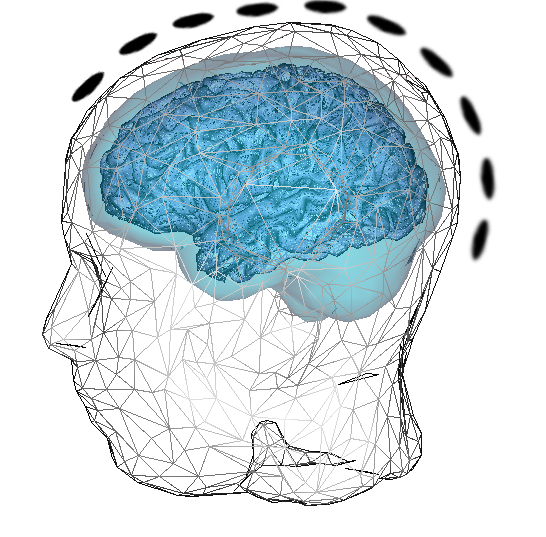
\includegraphics[height=9cm]{surf3.png}}

\noindent
Le problème direct consiste à estimer la valeur des potentiels et champs magnétiques qui seraient enregistrés \textbf{aux
capteurs} MEG/EEG étant donné une source d'activité.

\centerline{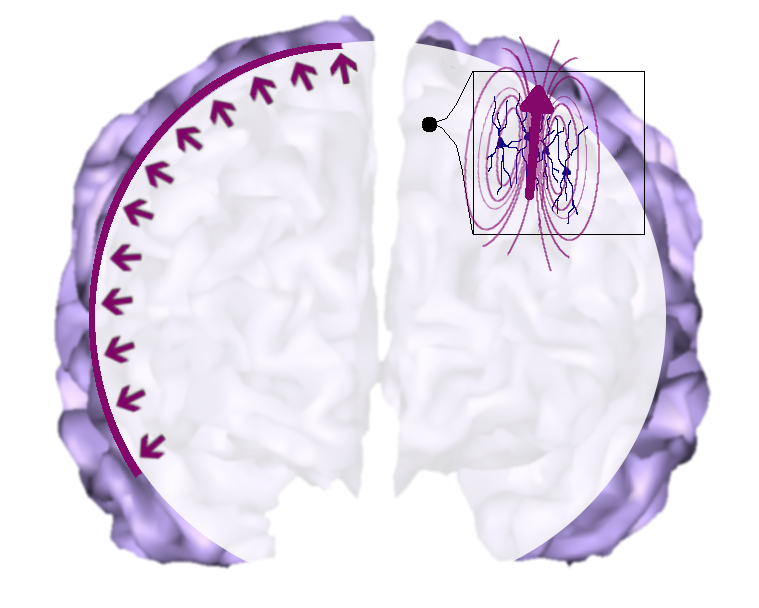
\includegraphics[height=10cm]{dipole.png}}

\noindent
\underline{Étape 1}~: on calcule le potentiel \textbf{sur la surface la plus externe} de la modélisation qui est en général le
scalp.  Soit $\mathbf{X}$ la matrice des potentiels en chaque points de la surface la plus externe. Par la méthode des éléments
frontières symétrique (voir thèse de Geoffray Adde), le calcul de $\mathbf{X}$ peut se ramener à la résolution du système
suivant~:
\[
    \mathbf{LHS} . \mathbf{X} = \mathbf{RHS}
\]
($\mathbf{LHS}$~: Left Hand Side member; $\mathbf{RHS}$~: Right Hand Side member)\\
Voir points \ref{sect: command assemble lhs}, \ref{sect: command assemble rhs} et \ref{sect: command invert lhs}.

\medskip

\noindent
\underline{Étape 2}~: on doit passer des potentiels calculés sur la dernière surface à ce qu'ils pourraient être \textbf{sur les
capteurs}. Il s'agit d'une application linéaire de la forme~:\\
\[
    \left[ \mbox{valeur aux capteurs} \right] =
    \left[ \mbox{matrice de passage} \right] \times \left[ \mbox{valeurs sur le scalp} \right] \mbox{dans le cas de l'EEG.}
\]
Et il faut rajouter la contribution de la position et de l'orientation des sources dans le cas de la MEG.\\
Voir point \ref{sect: command assemble sensors}.

\medskip

\noindent
\underline{Étape 3}~: on assemble la matrice liant \textbf{la position et l'orientation} des sources aux capteurs. Cette matrice
est appelée matrice de gain et notée $\mathbf{G}$~: on calcule la matrice de gain $\mathbf{G}$ (point \ref{sect: command gain})
qui, appliquée à une matrice reflétant l'\textbf{activation} des sources, nous donnera la solution du problème direct (point
\ref{sect: command direct}).
